\section{HtmlTag Class Reference}
\label{classHtmlTag}\index{HtmlTag@{HtmlTag}}
{\tt \#include $<$htmltag.h$>$}

Inheritance diagram for HtmlTag::\begin{figure}[H]
\begin{center}
\leavevmode
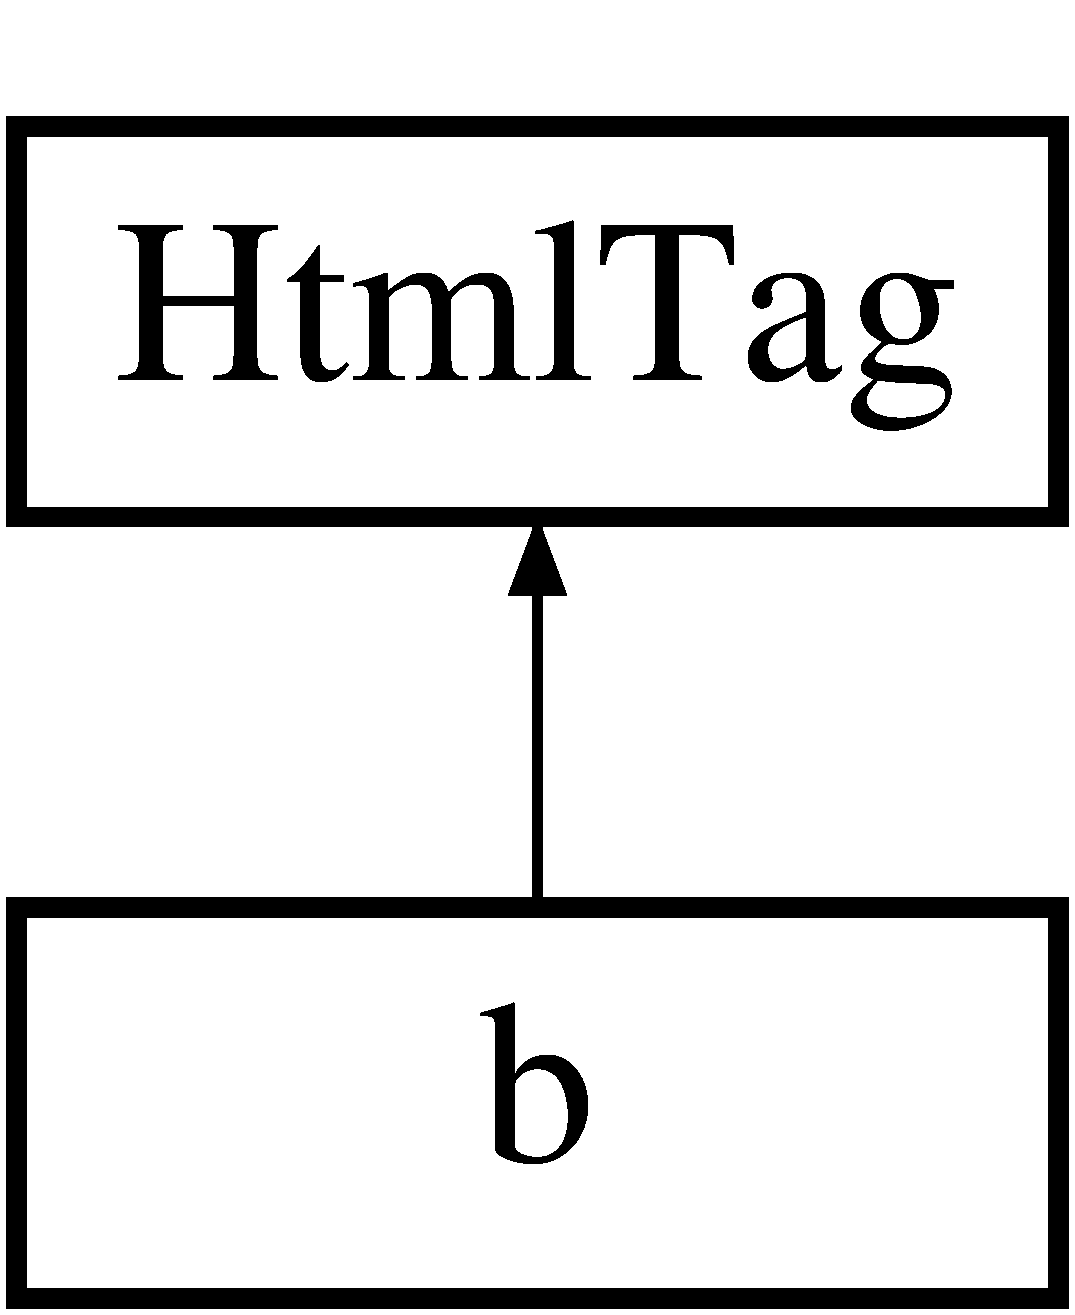
\includegraphics[height=2cm]{classHtmlTag}
\end{center}
\end{figure}
\subsection*{Public Member Functions}
\begin{CompactItemize}
\item 
\textbf{HtmlTag} (bool tagType=TAG\_\-PAIR)\label{classHtmlTag_62eb3105ee2592c4564cba840bf5dffb}

\item 
\textbf{HtmlTag} (const string \&tagName, bool tagType=TAG\_\-PAIR)\label{classHtmlTag_0076758379d841b014185a0baf664ba2}

\item 
void \textbf{setTagName} (const string \&tagName)\label{classHtmlTag_b175e70bde14ba15d160c7361fc08cde}

\item 
const string \& \textbf{getTagName} () const \label{classHtmlTag_46a1b30ccc0ee7e2a2942dd0d42b5a46}

\item 
virtual {\bf HtmlTag} \& \textbf{setAttr} (const string \&key, const {\bf Var} \&val)\label{classHtmlTag_6a1edcd9d1b0e3c3fab774f6874feb50}

\item 
virtual {\bf Var} \textbf{getAttr} (const string \&key) const \label{classHtmlTag_ab12ea73f5395b06873fc0d65b008a9f}

\item 
virtual {\bf HtmlTag} \& \textbf{removeAttr} (const string \&key)\label{classHtmlTag_dbb6d35fc0e7ea11a8e9b850884a4fa7}

\item 
virtual {\bf HtmlTag} \& \textbf{setId} (const {\bf Var} \&val)\label{classHtmlTag_3fadb90a3435758cebad17dd6c4e2d7a}

\item 
virtual {\bf HtmlTag} \& \textbf{setClass} (const {\bf Var} \&val)\label{classHtmlTag_7a6a5a4479f7e67f0796e3bc7c67b4d9}

\item 
virtual {\bf HtmlTag} \& \textbf{setName} (const {\bf Var} \&val)\label{classHtmlTag_43f09e229a49a26bb54425d84339c5c9}

\item 
virtual {\bf Var} \textbf{getId} () const \label{classHtmlTag_1698a6303bda5226627b0291c1da7b27}

\item 
virtual {\bf Var} \textbf{getClass} () const \label{classHtmlTag_6852dbba1ff504500796eb22f67d25b2}

\item 
virtual {\bf Var} \textbf{getName} () const \label{classHtmlTag_c1d2797c8240cfed348d942bb5928a28}

\item 
virtual string \textbf{open} () const \label{classHtmlTag_c259f32d68385a8fe05b45211ac22a9e}

\item 
virtual string \textbf{close} () const \label{classHtmlTag_39c5f9b8f582fb4e3e502c3556ef63e5}

\item 
string \textbf{autoComplete} () const \label{classHtmlTag_de0a8b993d7dae6ed9b394c2307cf817}

\end{CompactItemize}
\subsection*{Public Attributes}
\begin{CompactItemize}
\item 
char \textbf{quoteType}\label{classHtmlTag_997be48566824cbb7dfe293c684406e6}

\end{CompactItemize}
\subsection*{Protected Member Functions}
\begin{CompactItemize}
\item 
virtual string \textbf{makeAttr} () const \label{classHtmlTag_0e2c807c620d5036e1075271a0b8c440}

\end{CompactItemize}
\subsection*{Private Attributes}
\begin{CompactItemize}
\item 
bool \textbf{mTagType}\label{classHtmlTag_0f613e3d7d43595fa69175ac9a966b13}

\item 
string \textbf{mTagName}\label{classHtmlTag_9d633cde7073067759c261135fb592da}

\item 
{\bf ParamsMap} \textbf{mAttr}\label{classHtmlTag_895fa5e2b887e674df0710259dd83b56}

\end{CompactItemize}
\subsection*{Friends}
\begin{CompactItemize}
\item 
ostream \& \textbf{operator$<$$<$} (ostream \&o, const {\bf HtmlTag} \&t)\label{classHtmlTag_378170d98d050945592ea3afc7adb9f0}

\end{CompactItemize}


\subsection{Detailed Description}
\begin{Desc}
\item[Author:]Neel Basu $<$neel$>$ \end{Desc}


The documentation for this class was generated from the following files:\begin{CompactItemize}
\item 
htmltag.h\item 
htmltag.cpp\end{CompactItemize}
